\documentclass{jarticle}
\usepackage[dvipdfmx]{graphicx}
\usepackage[dvipdfmx]{color}
%\usepackage {okumacro}

%\usepackage{amsmath} % さまざまな数式を用いるための設定
%\usepackage{amsthm}
%\usepackage{mathrsfs}
%\usepackage[dvipdfmx]{pict2e}
\usepackage[dvipdfmx]{hyperref}
\usepackage{pxjahyper}		%日本語設定
%\hypersetup{bookmarks=true}
%\hypersetup{bookmarksopen=true}
%\usepackage{emath}
%\usepackage{amsfonts}%白抜きbold作成
%\usepackage{url}%urlの記述
%\usepackage{makeidx} % 索引作成
%\usepackage{lscape} %landscaoeのときにpdfを反転する.
%\usepackage{longtable}	%tableに改頁

%\usepackage{tikz}%tikzを発動!
%\usepackage{tikz-cd}
%\usetikzlibrary{positioning}%
%\usetikzlibrary{matrix}
%\usepackage[abbrev]{amsrefs}


% ######## measure #########
% # mm = 1mm = 2.85pt      #
% # cm = 10mm = 28.5pt     #
% # in = 25.4mm = 72.27pt  #
% # pt = 0.35mm = 1pt      #
% # em = width of [M]      #
% # ex = height of [x]     #
% # zw = width of [Kanji]  #
% # zh = height of [Kanji] #
% ##########################
% ##################### Portrait Setting #########################
% # TOP = 1inch + \voffset + \topmargin + \headheight + \headsep #
% #     = 1inch + 0pt + 4pt + 20pt + 18pt (default)              #
% # BOTTOM = \paperheight - TOP -\textheight                     #
% ################################################################
\setlength{\textheight}{\paperheight}   % 紙面縦幅を本文領域にする(BOTTOM=-TOP)
\setlength{\topmargin}{4.6truemm}       % 上の余白を30mm(=1inch+4.6mm)に
\addtolength{\topmargin}{-\headheight}  %
\addtolength{\topmargin}{-\headsep}     % ヘッダの分だけ本文領域を移動させる
\addtolength{\textheight}{-60truemm}    % 下の余白も30mm(BOTTOM=-TOPだから+TOP+30mm)
% #################### Landscape Setting #######################
% # LEFT = 1inch + \hoffset + \oddsidemargin (\evensidemargin) #
% #      = 1inch + 0pt + 0pt                                   #
% # RIGHT = \paperwidth - LEFT - \textwidth                    #
% ##############################################################
\setlength{\textwidth}{\paperwidth}     % 紙面横幅を本文領域にする(RIGHT=-LEFT)
\setlength{\oddsidemargin}{-0.4truemm}  % 左の余白を25mm(=1inch-0.4mm)に
\setlength{\evensidemargin}{-0.4truemm} %
\addtolength{\textwidth}{-50truemm}     % 右の余白も25mm(RIGHT=-LEFT)

%%%%%%%%%%%%%%%%%%%%%%%%%%%%%%%%%%%%%%%%%%%%%%%%%%%%%%%%%%%%%
%↑priamble
%
%%%%%%%%%%%%%%%%%%%%%%%%%%%%%%%%%%%%%%%%%%%%%%%%%%%%%%%%%%%%%
\begin{document}

\begin{flushleft}

  { \fontsize{24pt}{0pt}\selectfont
    Yokubari道路セットの取り扱い説明書
  }
	\\
\vspace{3pt}
	{ \fontsize{12pt}{0pt}\selectfont
		How to use Yokubari roads set
	}
	\\
\vspace{15pt}
	{ \fontsize{18pt}{0pt}\selectfont
		著者: あのKTOK
	}
	\\
\vspace{2pt}
	{ \fontsize{12pt}{0pt}\selectfont
		Author: ano KTOK
	}
	\\
\vspace{15pt}
	{ \fontsize{12pt}{0pt}\selectfont
		Date: 2020/Feb./14
	}
\end{flushleft}

\vspace{15pt}
\begin{flushleft}
  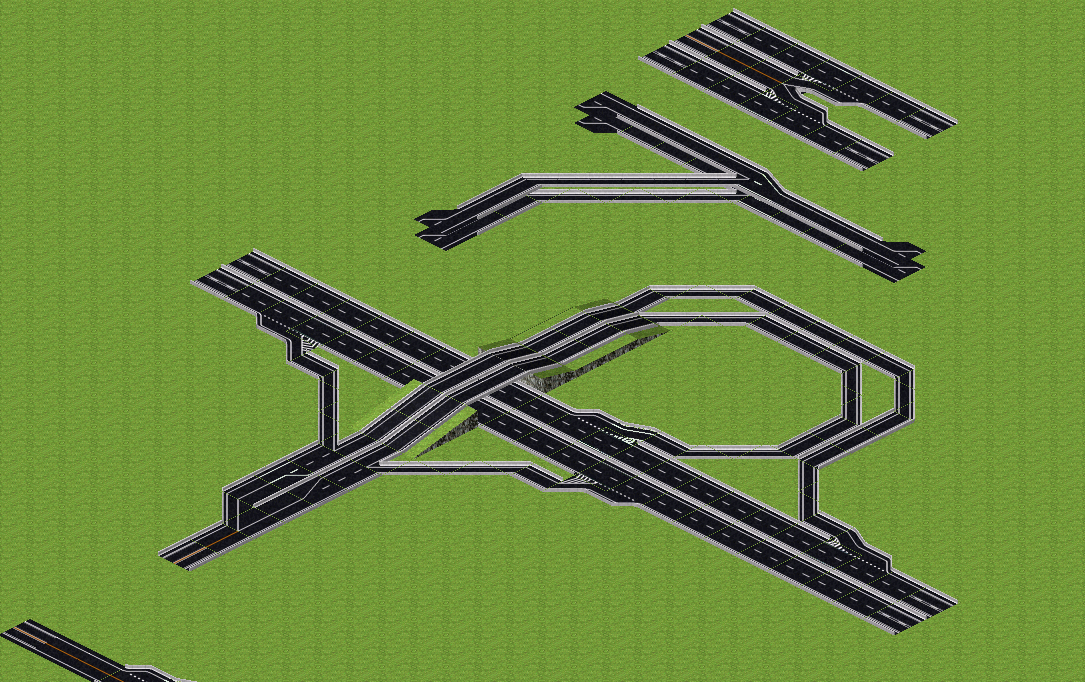
\includegraphics[width = 15cm]{picture/20210207app1.png}
\end{flushleft}


\newpage

\renewcommand{\contentsname}{目次 / Index}
\tableofcontents

\newpage

\part{日本語版}

\section{はじめに}
本プロジェクトは都市開発・輸送シミュレーションゲームであるSimutransにアドオンを追加することで、道路をメインにかつて無いリアリティーをもってインフラを再現することを目的とする。

これらアドオンは全て統一規格のもとに開発され、相互に組み合わせることで拡張性と景観表現の自由度を向上させる。
この一種のモジュール構造ともいえるような実装方法をとった結果、景観表現力と引き換えに極端にユーザビリティを犠牲にせざるを得なかったため、万人に受け入れられるものではない。
しかし、それでもなお、リアリティーを追求してやまないインフラに拘りを持つ同志に利用していただければこれ幸いである。

\subsection*{前提知識}
 Simutransの基本的な操作方法(道路の引き方、消し方)、アドオンの導入の仕方は既知とします。

\subsection*{Pak file}
 128standard版は128standard/paksetに置いています。(予定)

 128extended版は\href{https://github.com/anoKTOK/Yokubari_roads_set_ver_anoKTOK/tree/main/128extended/pakset}{128extended/pakset}に置いています。

\subsection*{ja.tab, en.tab}
128standard版は128standard/pakset/textに置いています。(予定)

128extended版は\href{https://github.com/anoKTOK/Yokubari_roads_set_ver_anoKTOK/tree/main/128extended/pakset/text}{128extended/pakset/text}に置いています。


\subsection*{ライセンス}
特記なき限り本リポジトリ内のpak及びdat, pngファイルは
"クリエイティブ・コモンズ 表示 - 非営利 - 継承 4.0 国際 ライセンス"
によって許諾されています。ライセンスの内容を知りたい方はコモンズ証をご確認ください。

コモンズ証:\href{http://creativecommons.org/licenses/by-nc-sa/4.0/deed.ja}{http://creativecommons.org/licenses/by-nc-sa/4.0/deed.ja}

リーガルコード:\href{http://creativecommons.org/licenses/by-nc-sa/4.0/legalcode}{http://creativecommons.org/licenses/by-nc-sa/4.0/legalcode}

\subsection*{注意書き}

\begin{description}
  \item[(1)]
    本paksetの中には製作者がKTOK以外に関係する方が居られます。引用する際は各パックセットの著者・編集者(copyright)をご確認の上、参照下さい。
  \item[(2)]
    pak更新にて、前のデータが読み込めないということはないように配慮します。しかし、パックセットによっては、描画の変更があります。
\end{description}

\subsection*{連絡}
万が一、製品に不具合がございましたら、ご連絡下さい。 ただし、本説明書を読んでからでお願いいたします。 場合によっては連絡できないことがありますのでご了承下さい。

\href{https://twitter.com/ano_KTOK_}{@ano\_KTOK\_}

\newpage

\section{アドオン一覧}



\subsubsection*{道路ツール / Road Tools}

\begin{flushleft}
  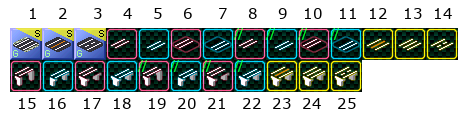
\includegraphics{picture/menu-1-1.png}
\end{flushleft}
\begin{tabular}{rll}
  番号 & 道路 & 詳細 \\
  & 一般道 & 地上 \\
  1 & 2車線 市道 & \\
  2 & 2車線 黄線  & \\
  3 & 2車線 破線 & \\
  & 高速道路 & 地上 \\
  4 & 1車線 & 奥 角が丸い \\
  5 & 1車線 & 手前 角が丸い \\
  6 & 1車線 & 奥 幅広路肩 角が丸い \\
  7 & 1車線 & 手前 幅広路肩 角が丸い \\
  8 & 1車線 & 奥 角が直線 and 分岐奥\\
  9 & 1車線 & 手前 角が直線 and 分岐手前\\
  10 & 1車線 & 奥 幅広路肩 角が直線  and 分岐奥\\
  11 & 1車線 & 手前 幅広路肩 角が直線 and 分岐手前\\
  12 & 2車線 黄線 & \\
  12 & 2車線 白線 & \\
  13 & 2車線 破線 & \\
  & 高速道路 & 高架 \\
  14 & 1車線 & 奥 角が丸い \\
  15 & 1車線 & 手前 角が丸い \\
  16 & 1車線 & 奥 幅広路肩 角が丸い \\
  17 & 1車線 & 手前 幅広路肩 角が丸い \\
  18 & 1車線 & 奥 角が直線 and 分岐奥\\
  19 & 1車線 & 手前 角が直線 and 分岐手前\\
  20 & 1車線 & 奥 幅広路肩 角が直線 and 分岐奥 \\
  21 & 1車線 & 手前 幅広路肩 角が直線 and 分岐手前\\
  22 & 2車線 黄線 & \\
  23 & 2車線 白線 & \\
  24 & 2車線 破線 & \\
\end{tabular}

\vspace{5pt}
ライム色(明るい黄緑色)の//が付いているものは角が直線になってます。

\newpage

\subsubsection*{市電/軽便鉄道ツール / Trams/light rail Tools}
\begin{flushleft}
  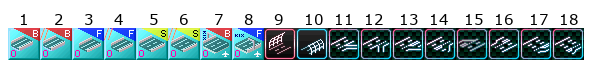
\includegraphics{picture/menu-2-1.png}
\end{flushleft}
\begin{tabular}{rll}
  番号 & 道路 & 詳細 \\
  1 & 1車線 & 奥 角が丸い \\
  2 & 1車線 & 奥 角が直線 and 行き止まりが2車線から1車線 \\
  3 & 1車線 & 手前 角が丸い \\
  4 & 1車線 & 手前 角が直線 and 行き止まりが2車線から1車線 \\
  5 & 2車線 & 角が丸い \\
  6 & 2車線 & 角が直線 and 2車線から1+1車線 分岐 合流 \\
  7 & 2車線 & 側壁 関空連絡橋仕様 奥 角が丸い \\
  8 & 2車線 & 側壁 関空連絡橋仕様 手前 角が丸い \\
  9 & 2車線 & 曲面防音壁 奥\\
  10 & 2車線 & 曲面防音壁 手前\\
  11 & 2車線 + 登板車線 & 本線2車線 - 補助1車線 合流\\
  12 & 2車線 + 登板車線 & 本線2車線 - 補助1車線 分岐\\
  13 & 3車線化 & 本線2車線 - 補助2車線 合流\\
  14 & 3車線化 & 本線2車線 - 補助2車線 分岐\\
  15 & & 本線2車線 - 補助1車線 右側合流 and 2車線から1車線\\
  16 & & 本線2車線 - 補助1車線 右側分岐 and 2車線から1車線\\
  17 & & 本線3車線 - 補助1車線 合流\\
  18 & & 本線3車線 - 補助1車線 分岐\\
\end{tabular}

\vspace{5pt}
朱色の//が付いているものは角が直線になってます。//が付いている者同士と相性がいいです。


\newpage

\section{組み合わせ}




\newpage

\part{English version}

\section{Introduction}

The aim of this project is to add addons to Simutrans, an urban development and transportation simulation game, to recreate infrastructure with unprecedented realism, mainly roads.

All of these addons are developed under a unified standard and can be combined with each other to improve scalability and flexibility of landscape expression.
As a result of this kind of modular implementation, we had to sacrifice extreme usability in exchange for the ability to express the scenery, so it is not something that can be accepted by everyone.
Nevertheless, we hope if it could be used by comrades who are concerned about infrastructure and who are still in pursuit of reality.

\end{document}
